\chapter{Diagrammes de classes}

Cette partie contient tous les diagrammes de classes décrivant l'architecture du site web. Certains diagrammes peuvent être aussi accompagnés des quelques explications.
 
\newpage

\section{Diagrammes de classes de l'application cakephp}

\subsection{Contrôleurs}

\begin{figure}[H]
	\begin{center}\fbox{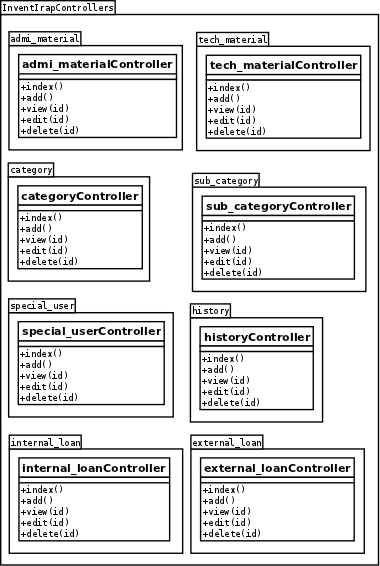
\includegraphics[]{images/controller.png}}\end{center}
	\caption{Contrôleurs du site web}
\end{figure}

\subsection{Vues}

\begin{figure}[H]
	\begin{center}\fbox{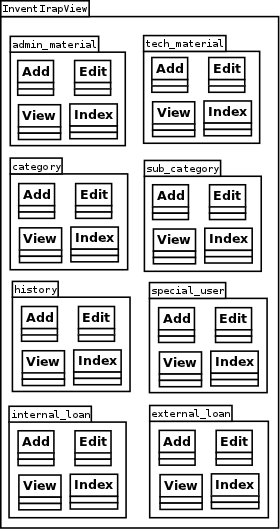
\includegraphics[]{images/view.png}}\end{center}
	\caption{Vues du site web}
\end{figure}

Les classes définies dans ce diagramme sont en fait des fichier .cpt qui ne représentent que de simples fichiers php. Ils permettent de définir les vues de l'application.

\subsection{Modèles}

\begin{figure}[H]
	\begin{center}\fbox{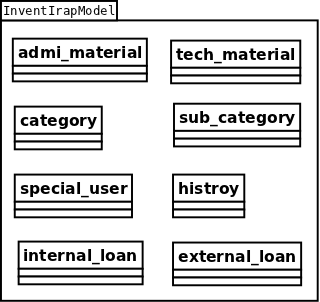
\includegraphics[]{images/model.png}}\end{center}
	\caption{Modèle du site web}
\end{figure}

Les classes définies dans ce diagramme ne contiennent qu'un simple tableau qui permet d'ajouter des contraintes sur la valeur des champs qui sont édités.
